\section{Experiments}
\label{sec:results}

Section~\ref{sec:mechanism} argues that probe agreement cannot make a stop safe
on its own, because the probes are not independent readings. The experiments here
establish that this is not a matter of tuning: we search the rule space
exhaustively and under commitment, and find nothing that escapes it.

We first confirm the phenomenon the paper turns on---intermediate consensus is
non-terminal (\S\ref{sec:exp-fc})---then report the preregistered sweep and its
central negative result: \emph{no} consensus rule is both safe and saving
(\S\ref{sec:exp-sweep}). We then show the failure is specific to the
\emph{signal}, not to early exit, by sweeping a non-consensus method (DEER)
through the identical pipeline and gates and finding that it \emph{does} clear
them (\S\ref{sec:exp-deer}); a released consensus stopper, CertaIndex (CoT),
shows the same failure at its default setting (\S\ref{sec:exp-prior}). Finally we confirm the frontier
out of distribution (\S\ref{sec:exp-heldout}).

\subsection{Non-Terminal Agreement}
\label{sec:exp-fc}
We log a dense probe stream for every \textsc{MATH}500 problem under \dsseven{}
at the main $16$K/$32$K budgets (all $500$ problems, three seeds; $1{,}500$
trajectories), never intervening---the probe is a separate forward pass that only
observes the main trajectory (full setup in Appendix~\ref{sec:appendix-fc})---and
read off four facts.

\textbf{(1) Final agreement is reliable; early agreement is not.} By the time a
trajectory finishes, agreement does track correctness: \emph{cumulative}
agreement across all probes is $97.8\%$ correct ($186$ trajectories reach it), and
even the final five-probe \emph{window} is $90.4\%$ correct ($1{,}205$). But an
online rule cannot wait for the end---it fires the \emph{first} time probes
agree, mid-trajectory, where the answer is far from settled (facts 2--4). The
operative question is not whether \emph{final} consensus is trustworthy, but
whether \emph{early} consensus is---and it is not.
\textbf{(2) Recovery is common.} Of the $1{,}148$ trajectories whose \emph{first}
probe is wrong, $89.1\%$ eventually flip to correct; of the $736$ that formed a
three-probe consensus \emph{different} from their final answer, $84.2\%$ ended up
correct.
\textbf{(3) Later consensus is worse.} Consensus formed before $512$ tokens is
$91.0\%$ correct, but consensus forming only after $2048$ tokens is $71.6\%$
correct---hard problems converge slowly \emph{and} to worse answers.
\textbf{(4) The cost lands at the stop.} A naive stop (first three consecutive
agreeing, certain, non-empty probes) fires on $1{,}477/1{,}500$ trajectories and
commits to answers correct only $50.5\%$ of the time, whereas letting those same
problems run to completion reaches $90.7\%$: a $40.2\pp$ loss.\footnote{A
simplified heuristic, \emph{not} the CertaIndex (CoT) rule (\S\ref{sec:exp-prior});
it fires early because the first stable, certain agreement is typically a
mid-trajectory placeholder. The swept rules below and the mechanism of
Section~\ref{sec:mechanism} quantify the same directional accuracy tax across the
full rule space.}

Figure~\ref{fig:consensus-pos} shows where this cost is concentrated. Expressing
the moment consensus first forms as a \emph{fraction} of each trajectory's own
length---which controls for problem difficulty---half of all consensuses form
within the first tenth of the trajectory, and there the answer they commit to is
correct only $27.5\%$ of the time against $85.2\%$ for the same problems run to
completion. The gap narrows as consensus forms later, but an online rule cannot
choose to wait: it fires when agreement first appears, which is precisely where
agreement is least informative.

A good stopping rule must therefore be much more than ``agreement.'' The rest of
this section asks whether the \emph{best possible} such rule, drawn from a large
preregistered space, can be both safe and economical.

\begin{figure}[t]
  \centering
  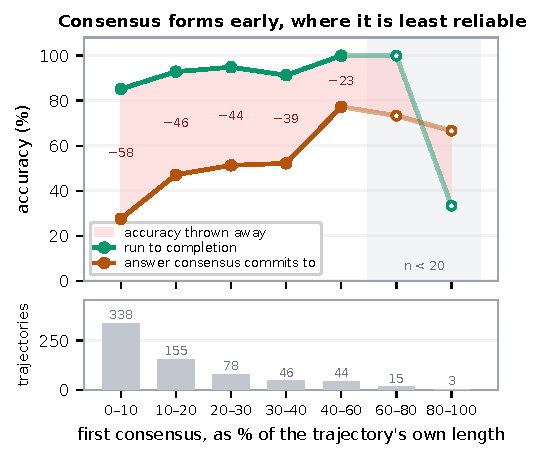
\includegraphics[width=\columnwidth]{figures/gen/fig_consensus_pos.pdf}
  \caption{\textbf{Consensus forms early, where it is least reliable.} For each
  dev-split trajectory we take the first window of three agreeing non-empty
  probes and ask two things: is that answer correct, and would the same problem
  have been correct if left to run? Position is a fraction of the trajectory's
  \emph{own} length, so $500$ tokens into a $600$-token trajectory counts as
  late and $500$ into a $16$K one does not. Consensus forms in $679$ of $684$
  trajectories, half within the first tenth; the shaded gap is the accuracy a
  stop at that moment throws away. Open markers mark bins with fewer than $20$
  trajectories; the final bin ($n{=}3$) should not be read.}
  \label{fig:consensus-pos}
\end{figure}

\subsection{Sweep Results}
\label{sec:exp-sweep}
We replay all $3{,}520$ consensus rules on the frozen trajectories and aggregate
to per-environment metrics---$126{,}720$ rows $=3{,}520$ rules $\times$ $18$
environments $\times$ $2$ splits (train, dev)---then, per rule, its total (macro)
accuracy drop and net token saving (accounting of Section~\ref{sec:accounting}).
Applying the preregistered gates yields the negative result that
Section~\ref{sec:mechanism} explains.

The outcome holds across environments: across all $126{,}720$ rule--environment
evaluations accuracy strictly \emph{falls} in $64.9\%$ and strictly \emph{rises}
in only $10.5\%$ (unchanged in $24.6\%$), for a mean drop of $13.0\pp$; over rules
the total dev drop has median $13.2\pp$ and a minimum of $0.81\pp$.
\textbf{Not one of the $3{,}520$ rules clears any gate.} The reason is the shape
of the trade-off, which Figure~\ref{fig:ws-heatmap} reads directly off the
sweep's own two axes: staying accurate and saving tokens are
in direct tension. Only $40$ rules keep the total drop at or below the
conservative $1.0\pp$ cap, and the most any of them saves is
$0.2\%$---far under the $10\%$ floor; conversely, the first rule to save $10\%$
already costs $2.66\pp$, saving $20\%$ costs $6.17\pp$, and saving $30\%$ costs
$11.8\pp$. Crucially, the sweep now includes \emph{large} windows (up to
$W{=}30$): these do buy low accuracy drop, but only by stopping so late that net
saving collapses to zero. No setting of the consensus signal escapes the
trade-off. Figure~\ref{fig:ws-heatmap} makes this a property of the whole
surface rather than of the frontier's edge: read cell by cell, the safest rule
available at each $(W,s)$ approaches the $1\pp$ cap only as the saving it buys
approaches zero, while every cell that saves substantially costs several points.
No cell clears the conservative gate.

\begin{figure*}[t]
  \centering
  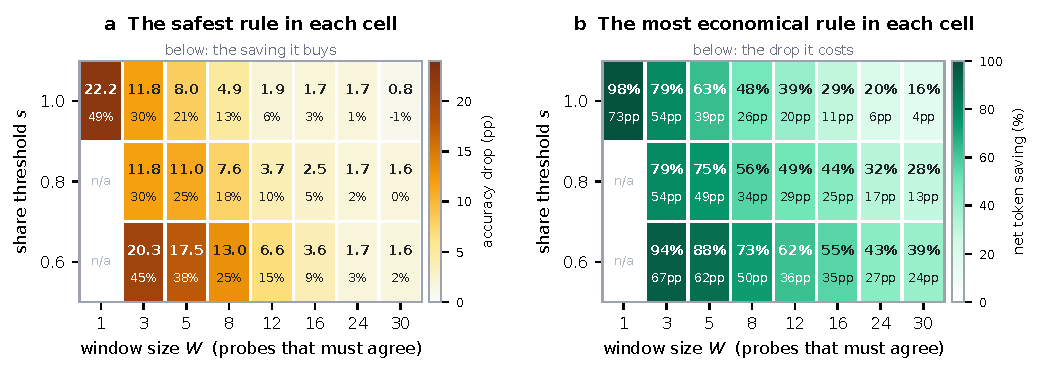
\includegraphics[width=\textwidth]{figures/gen/fig_ws_heatmap.pdf}
  \caption{\textbf{The safe-and-saving corner is empty across the entire rule
  space.} Dev split, macro-averaged over the $18$ environments. Each cell holds
  the $160$ rules that share its $(W,s)$ and differ only in the operational
  knobs, summarised by the two members a gate interrogates.
  \textbf{(a)} the cell's \emph{safest} rule: colour is its accuracy drop and
  the number beneath is the saving that rule buys. Larger windows and stricter
  thresholds do drive the drop towards the $1.0\pp$ cap---but the saving falls
  with it, reaching $-1\%$ at $W{=}30$, $s{=}1.0$.
  \textbf{(b)} the cell's \emph{most economical} rule: colour is its net saving
  and the number beneath is the drop it costs. Substantial saving is available
  everywhere, at $4$--$73\pp$. A cell would be outlined in green if any of its
  rules cleared the conservative gate (drop $\leq 1.0\pp$ \emph{and} saving
  $\geq 10\%$); none is.}
  \label{fig:ws-heatmap}
\end{figure*}

\subsection{A Non-Consensus Signal}
\label{sec:exp-deer}
The same gates are cleared, comfortably, by a rule that does \emph{not} read probe
agreement. Sweeping DEER's confidence threshold through the identical pipeline and
token accounting (Section~\ref{sec:schema}), its trial-answer-submit variant
passes all three operating points on dev: the conservative point loses only
$0.33\pp$ while saving $28.2\%$, the balanced point $1.03\pp$ at $29.6\%$, and the
token-efficient point $2.75\pp$ at $31.9\%$; at a stricter threshold it is
accuracy-neutral ($-0.06\pp$) while still saving $20.8\%$. Early exit is
therefore not impossible; the consensus \emph{signal} is what cannot make it
safe (Table~\ref{tab:main}).

\begin{table}[t]
  \centering\small
  \setlength{\tabcolsep}{4pt}
  \begin{tabular}{lccc}
    \toprule
    Method & Acc. & $\Delta$acc & Net \\
           &      & (macro)     & saving \\
    \midrule
    Full generation & $82.5\%$ & --- & $0\%$ \\
    \midrule
    Consensus (drop$\le1.0$)  & $81.6\%$ & $-0.9\pp$  & $+0.2\%$ \\
    Consensus (save$\ge10\%$) & $79.9\%$ & $-2.7\pp$  & $+10.7\%$ \\
    \midrule
    DEER (conservative)      & $82.5\%$ & $-0.33\pp$ & $+28.2\%$ \\
    DEER (balanced)          & $81.9\%$ & $-1.03\pp$ & $+29.6\%$ \\
    DEER (token\_eff.)       & $80.1\%$ & $-2.75\pp$ & $+31.9\%$ \\
    \bottomrule
  \end{tabular}
  \caption{Dev operating points (macro over $18$ environments). No consensus rule
  is simultaneously safe ($\le1.0\pp$) and saving ($\ge10\%$): capping the drop
  forces saving to near zero, and demanding saving forces a large drop. DEER,
  reading a non-consensus signal, clears all three gates on the same trajectories
  under the same accounting.}
  \label{tab:main}
\end{table}

\subsection{CertaIndex (CoT) at Its Default}
\label{sec:exp-prior}
The sweep covers rules we constructed; a released method lets us see where a
default setting lands. We reproduce two prior stoppers in a common harness---the
same frozen trajectories, the same token accounting.
\textbf{CertaIndex (CoT)} \citep{dynasor_certaindex} is the consensus stop for a
single chain of thought, reproduced from the released implementation at its
default \texttt{mid} setting: stop once three consecutive probes give the same
non-empty answer and none hedges. We use the authors' probe prompt and probe
schedule, so this is their rule as shipped, not a variant of ours.
\textbf{DEER} \citep{deer} here is the readout reproduction (the stronger
trial-answer-submit variant is what we swept in \S\ref{sec:exp-deer}).

Two scope notes. First, CertaIndex's multi-path setting is ordinary
self-consistency: it measures entropy over answers from \emph{independently
sampled} trajectories, and nothing here bears on it. What we reproduce is the
single-trajectory case, where the same statistic is read over repeated probes of
one chain. Second, Table~\ref{tab:baselines} reports these reproductions on our
frozen trajectories and benchmarks; it is not a re-run of either paper's
end-to-end system, and the original CoT results were reported on an easier
benchmark, where intermediate answers settle sooner.

\begin{table*}[t]
  \centering\small
  \begin{tabular}{llccccc}
    \toprule
    Method & Model & Accuracy & $\Delta$acc & Fair token saving & Stop rate & Signal \\
    \midrule
    Full generation & \qweneight{}   & $85.4\%$ & --- & $0\%$ & $0\%$ & --- \\
    Full generation & \dsseven{} & $79.8\%$ & --- & $0\%$ & $0\%$ & --- \\
    \midrule
    CertaIndex (CoT) & \qweneight{}   & $15.3\%$ & $-70.1\pp$ & $90.1\%$ & $99.8\%$ & consensus \\
    CertaIndex (CoT) & \dsseven{} & $23.9\%$ & $-55.9\pp$ & $76.7\%$ & $98.7\%$ & consensus \\
    \midrule
    DEER       & \qweneight{}   & $86.2\%$ & $\mathbf{+0.8\pp}$ & $16.3\%$ & $41.4\%$ & boundary conf. \\
    DEER       & \dsseven{} & $74.9\%$ & $-4.8\pp$  & $20.2\%$ & $56.1\%$ & boundary conf. \\
    \bottomrule
  \end{tabular}
  \caption{Prior early-stoppers reproduced on our frozen trajectories (dev, macro
  over three benchmarks; probe tokens charged). \textbf{CertaIndex (CoT)} stops on
  almost every problem and stops early, and loses $56$--$70\pp$ while saving
  $77$--$90\%$ of tokens---the pattern \S\ref{sec:exp-fc} describes, at a single
  shipped operating point. \textbf{DEER}, reading boundary confidence rather than
  probe agreement, stays near full accuracy ($+0.8\pp$ on \qweneight{}) while
  still saving tokens. These are reproductions on our benchmarks, not the original
  papers' end-to-end numbers; Section~\ref{sec:mechanism} interprets the
  contrast.}
  \label{tab:baselines}
\end{table*}

At a $99.8\%$ stop rate and $70\pp$ lost, CertaIndex (CoT) lands where the swept
consensus frontier says a rule at that stop rate must land. This is a property of
the signal, not a defect of the implementation: it is the same trade-off
\S\ref{sec:exp-sweep} maps across the whole rule space, seen at one shipped
operating point. The DEER readout, reading a non-consensus signal on the same
trajectories, stays near full accuracy; the stronger trial-answer-submit variant
we swept turns that into a gate-clearing frontier (\S\ref{sec:exp-deer}). That
only the non-consensus signal survives is what we analyze in
Section~\ref{sec:mechanism}.

\subsection{Generalization}
\label{sec:exp-heldout}
We read the test split once (commitment~C3). Because the development result is that
\emph{no} consensus rule clears any gate, there is nothing to confirm by
re-selection; we ask whether the \emph{frontier} reproduces, ranking rules on dev
and measuring on test.

\paragraph{Held-out test split.}
Each consensus rule's total drop on test tracks its dev value closely
($r=0.98$). The split-invariant claim is the empty \emph{joint} gate:
\textbf{no consensus rule clears the conservative gate on both splits}---$0$ on
dev, and the $444$ rules admissible on \emph{test alone} are exactly the
in-sample winners the held-out split exists to reject (all fail on dev). DEER, by
contrast, remains admissible across splits: $3$ of its thresholds clear the
conservative gate on \emph{both} dev and test (and $5$ clear balanced on both),
so the cross-signal contrast is not a dev artifact.

\paragraph{Unseen scale ($4\times$) and architecture.}
Both unseen models are evaluated on the test split at three seeds ($45/46/47$;
nine environments each), so their gates are as well resolved as development's. On
\mbox{Distill-Qwen-32B}, never used in development, the consensus frontier
reproduces ($r=0.97$ against dev drop); on the held-out architecture and family
\mbox{DeepSeek-R1-Distill-Llama-8B} it reproduces at $r=0.94$.\footnote{The
Llama-8B trajectories were re-collected after correcting a chat-template defect
(a missing model-specific beginning-of-sequence token that degraded its
generations); the corrected model scores $\sim\!88\%$ on \textsc{MATH}500.} The
\emph{conservative} gate stays empty on every model---dev, $32$B, and Llama all
admit $0$ rules (the best rule under a $1.0\pp$ drop saves $0.6\%$ on $32$B and
$9.3\%$ on Llama). At the looser gates a scale effect appears: on the $4\times$
larger $32$B a few consensus rules become admissible in-sample ($4$ at balanced,
$6$ at token-efficient), reflecting that a bigger model's intermediate answers
stabilize somewhat earlier---but these are not the dev-selected rules (dev admits
none), and on the same-scale Llama architecture the gates stay empty
($0/0/0$). Consensus thus yields no rule that is safe-and-saving where it is
selected, on any model. DEER, swept identically on these unseen models,
\textbf{clears the gates on both}: on \mbox{Qwen-32B} it is accuracy-neutral at
the conservative point ($-0.24\pp$ while saving $32.4\%$, $\tau{=}0.97$) and on
\mbox{Llama-8B} it loses $0.67\pp$ at $26.7\%$ ($\tau{=}0.99$), passing all three
gates. Consensus is unsafe, and DEER safe-and-saving, across all four axes we
vary---benchmark, seed, $4\times$ scale, and architecture/family.

Figure~\ref{fig:split-transfer} shows the selection pipeline end to end. The
$478$ consensus rules that clear the conservative gate in-sample on train are
tracked onto dev and test as a band; the three dev-selected DEER thresholds are
tracked individually. On dev---the split the gate is applied on---not one of the
$478$ is admissible, and the joint gate is empty, while all three DEER points
stay inside on every split. The dev and test splits are not equally demanding:
the same $478$ rules have a median drop of $4.5\pp$ on dev but $0.6\pp$ on test,
an asymmetry driven by the two smallest environments (AMC23 and AIME24 under
\qweneight{}, $8$ and $6$ problems), which carry the same weight as a
$100$-problem environment under macro-averaging. This is why the claim is stated
jointly rather than per split: $364$ of the $478$ are admissible on test, but
they are exactly the in-sample winners a held-out split exists to reject, and
none of them is selectable from dev.

Per-model and per-benchmark views of the same data, together with an
\emph{oracle} upper bound---a perfect probe-based stop committing the earliest
correct probe, which sits at a negative drop of $2$--$5\pp$ at $40$--$80\%$
saving, far in a corner neither method reaches---are given in
Appendix~\ref{sec:appendix-pareto}.

\begin{figure*}[t]
  \centering
  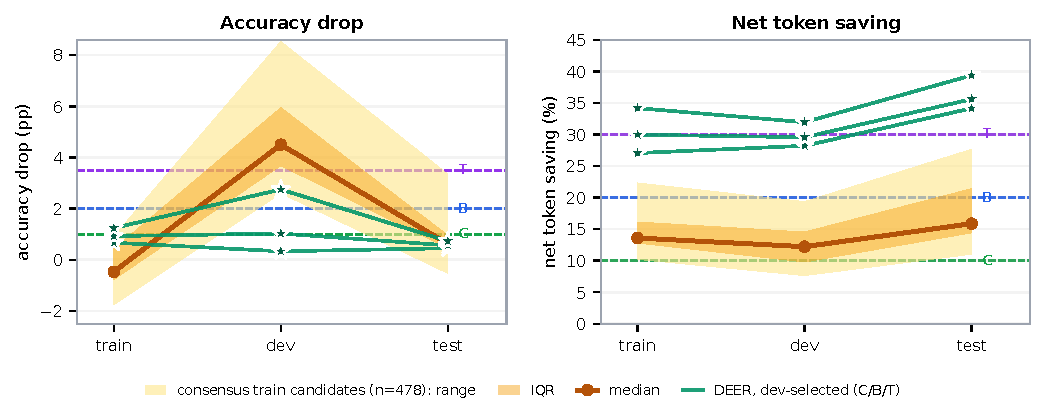
\includegraphics[width=\textwidth]{figures/gen/fig_split_transfer.pdf}
  \caption{\textbf{A rule must clear the gate on every split.} The $478$ amber
  rules are exactly those that clear the conservative gate \emph{in-sample on
  train}; drawing all $478$ would be unreadable, so we show their median,
  interquartile range and full range. Dashed lines mark all three preregistered
  gates (\textbf{C}onservative, \textbf{B}alanced, \textbf{T}oken-efficient);
  a rule must sit below them on the left and above them on the right. On dev,
  the split the gate is applied on, none of the $478$ does. Some recover on
  test, but a rule selected on dev is never among them: jointly, $0$ of $478$
  clear all three splits, against $3$ of $3$ for the DEER operating points
  selected on dev. Macro-averaged over $18$ environments per split; train and
  dev share seeds $42$--$44$ and differ only in problems, while test uses unseen
  problems and seeds $45$--$47$.}
  \label{fig:split-transfer}
\end{figure*}


